% Olympus v2 — flow start & bridge -> agent hand-off (generic, abstract)
% flow_agent_handoff.tex — one thin horizontal strip: a flow starts inside a
% non-descript emulated environment on a unique source port; the bridge sees
% the socket on :P, takes its fd, and execl()s into the agent, which then
% drives the flow directly via getsockopt / setsockopt on the inherited fd.
% Compile standalone:  pdflatex flow_agent_handoff.tex
\documentclass[tikz,border=2pt]{standalone}
\usepackage{tikz}
\usepackage{amssymb}
\usepackage{helvet}
\renewcommand{\familydefault}{\sfdefault}
\usetikzlibrary{arrows.meta,positioning,fit,backgrounds}

\begin{document}
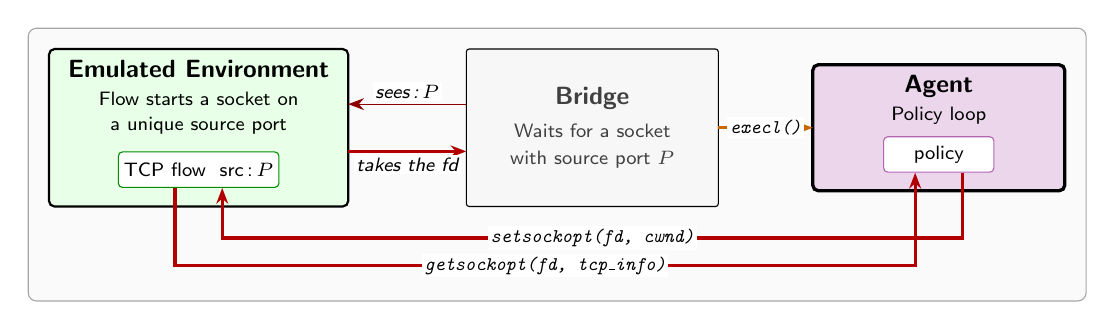
\begin{tikzpicture}[
  font=\small,
  >={Stealth[length=2mm]},
  proc/.style={draw,rounded corners=2pt,thick,minimum height=8mm,
               minimum width=24mm,align=center,fill=blue!7},
  net/.style={draw,rounded corners=2pt,thick,minimum height=8mm,
              minimum width=30mm,align=center,fill=green!9},
  agent/.style={proc,fill=violet!16,very thick},
  bridge/.style={draw,solid,thin,rounded corners=1pt,
                 minimum height=8mm,minimum width=24mm,align=center,
                 fill=black!3,text=black!75},
  flowbox/.style={draw,rounded corners=1.5pt,thin,draw=green!55!black,
                  fill=white,font=\scriptsize,inner sep=2pt,
                  minimum height=4.5mm},
  band/.style={draw,rounded corners=3pt,thin,draw=black!35,fill=black!2},
  subbox/.style={draw,rounded corners=1.5pt,thin,draw=violet!60,fill=white,
                 font=\scriptsize,inner sep=2pt,
                 minimum width=14mm,minimum height=4.5mm},
  data/.style={->,very thick,draw=red!70!black},
  tap/.style={->,thin,draw=red!55!black},
  cfg/.style={->,thick,draw=orange!80!black},
  lbl/.style={font=\scriptsize\itshape,fill=white,inner sep=1pt},
]

% ---- left: the environment, any emulated network, one flow on port P ----
\node[net,minimum width=38mm,minimum height=20mm] (env) at (0mm,0mm) {};
\node[align=center,anchor=north,inner sep=0pt] at ([yshift=-1.5mm]env.north)
     {\textbf{Emulated Environment}\\[-1pt]
      \scriptsize Flow starts a socket on\\[-2pt]
      \scriptsize a unique source port};
\node[flowbox,anchor=south] at ([yshift=2.5mm]env.south) (tcpflow)
     {TCP flow\ \ src\,:\,$P$};

% ---- middle: the bridge ----
\node[bridge,minimum width=32mm,minimum height=20mm] (bridgebox) at (50mm,0mm)
     {\textbf{Bridge}\\[1pt]
      \scriptsize Waits for a socket\\[-1pt]
      \scriptsize with source port $P$};

% ---- right: the agent it turns into, with its policy module ----
\node[agent,minimum width=32mm,minimum height=16mm] (agentbox) at (94mm,0mm) {};
\node[align=center,anchor=north,inner sep=0pt] at ([yshift=-1.5mm]agentbox.north)
     {\textbf{Agent}\\[-1pt]
      \scriptsize Policy loop};
\node[subbox,anchor=south] at ([yshift=2.5mm]agentbox.south) (policy)
     {policy};

% backdrop card around the whole hand-off
\begin{scope}[on background layer]
  \coordinate (loopbot) at (45mm,-19.5mm);
  \node[band,fit=(env)(bridgebox)(agentbox)(loopbot),inner sep=2.5mm]
       (backdrop) {};
\end{scope}

% the bridge sees the socket on :P and takes its fd
\draw[tap]  (34mm,3mm)  -- node[lbl,above=0.3mm]{sees\,:\,$P$}   (19mm,3mm);
\draw[data] (19mm,-3mm) -- node[lbl,below=0.3mm]{takes the fd} (34mm,-3mm);

% exec: the bridge becomes the agent
\draw[cfg,very thick] (66mm,0mm)
      -- node[lbl]{\texttt{execl()}} (78mm,0mm);

% control loop on the inherited socket: policy <-> tcp flow, routed under
% the strip with nested orthogonal lines
\coordinate (setline) at (0mm,-14mm);
\coordinate (getline) at (0mm,-17.5mm);

\draw[data] ([xshift=3mm]policy.south)
      -- ([xshift=3mm]policy.south |- setline)
      -- node[lbl]{\texttt{setsockopt(fd, cwnd)}}
         ([xshift=3mm]tcpflow.south |- setline)
      -- ([xshift=3mm]tcpflow.south);

\draw[data] ([xshift=-3mm]tcpflow.south)
      -- ([xshift=-3mm]tcpflow.south |- getline)
      -- node[lbl]{\texttt{getsockopt(fd, tcp\_info)}}
         ([xshift=-3mm]policy.south |- getline)
      -- ([xshift=-3mm]policy.south);

\end{tikzpicture}
\end{document}
